% !TEX root = template.tex

\lstset{
	basicstyle=\small,
	language=C
}

\section{Obtaining a Roofline Model}

\subsection{Machine 1}

\subsubsection{Theoretical Peak Performance}

\subsubsection{STREAM or NUMA-STREAM}

\subsubsection{Roofline Plot}


\subsection{Machine 2 / Mars}

\subsubsection{Theoretical Peak Performance}

\subsubsection{STREAM or NUMA-STREAM}

\subsubsection{Roofline Plot}


\section{Performance of kmeans Kernel}

\subsection{Compilation Details}

\subsection{Obtain AI for kmeans}

\begin{table}[h]
\centering
\caption{\label{tab:ai_tab}Overview of AIs obtained for kmeans on Mars}
\begin{small}
\begin{tabular}{lllll}
\toprule
\#cores & file & Total GFLOPS & Total GBytes & AI (FLOPS/Byte) \\
\midrule
10 & 100 & 2.3 & 3.4 & 0.67 \\
...\\
80 & 100 & 1.3 & 3.4 & 0.38 \\
...\\
\bottomrule
\end{tabular}
\end{small}
\end{table}

\subsection{Roofline plots for entire kmeans application}

\subsection{Roofline plots with realistic ceiling for kmeans kernel}

We arrive at a realistic Ceiling as follows:

Start with the theoretical peak performance: 1280 GFlops

Take into account the lack of SIMD parallelism: 
$$\frac{1280 GFlops}{4} = 320 GFlops$$

Take into account the imbalance of MUL vs ADD operations:
$$\frac{320 GFlops}{2 Flop/Cycle} *1.5 Flop/Cycle = 240 GFlops$$

\subsection{Obtain AI for kmeans with the LIKWID marker API}

\begin{table}[h]
\centering
\caption{\label{tab:ai_tab}Overview of AIs obtained for kmeans on Mars}
\begin{small}
\begin{tabular}{lllll}
\toprule
\#cores & file & Total GFLOPS & Total GBytes & AI (FLOPS/Byte) \\
\midrule
10 & 100 & 2.3 & 3.4 & 0.67 \\
...\\
80 & 100 & 1.3 & 3.4 & 0.38 \\
...\\
\bottomrule
\end{tabular}
\end{small}
\end{table}

\subsection{Roofline plots with realistic ceiling for kmeans kernel only (with marker API)}

\subsection{Comparison and Discussion}
















\section{Maximum performance of the kmeans kernel}

The kernel of the \texttt{kmeans} algoirthm is in the \texttt{kmeans\_clustering} function.

The function is split into three main parts:
\begin{itemize}
	\item Initialization (happens once)
	\item In the main loop:
	\begin{itemize}
		\item Calculating membership to existing clusters for each point.
		\item Update clusters.
	\end{itemize}
\end{itemize}

We can safely ignore initialization for our performance consideration which leaves the main loop.

\newpage
\subsection{The Main Loop}

We can split the main loop again into three somewhat distinct parts.
\begin{itemize}
	\item In a parallel loop:
	\begin{itemize}
		\item Find the nearest cluster for each point.
		\item Collect partial updates on the position of clusters.
	\end{itemize}
	\item Reduce partial information and update positions of clusters 	
\end{itemize}

For our analysis we assume 5 clusters and 34 features which matches
the default of kmeans and our input datasets.

The only significant contributors here are the loops to find the nearest cluster and updating the cluster information.
For this reason we will look only at these inner loops and not at the rest of the main loop.


\subsubsection{Main loop:Finding the nearest cluster}
\begin{lstlisting}[caption={Inlined representation of find\_nearest\_point}]
for (i=0; i<nclusters; i++) {
float dist=0;
for (j=0; j<nfeatures; j++)
dist += (pt1[j]-clusters[i][j]) * (pt1[j]-clusters[i][j]);
if (dist < min_dist) {
min_dist = dist;
index    = i;
}
}
\end{lstlisting}
The kernel here is: \texttt{dist += (pt1[j]-pt2[j]) * (pt1[j]-pt2[j])}.\newline

We get 8
\footnote{Actually 12. But we can ignore the store of dist as it will be held in a register.}
byte of memory bandwith and three floating point operations.
Memory bandwith consists of 2 loads for each iteration.
Operations are two additions and one multiplication.
\footnote{Treating subtraction as addition.}
\footnote{While there are two subtractions in the code gcc will eliminate one through common subexpression elimination.}
\begin{itemize}
	\item Read: \texttt{pt1[j]}
	\item Read: \texttt{clusters[i][j]}
\end{itemize}

Immediatly obvious from the snippet above we get at least $nclusters * nfeatures$ iterations.
With one call to \texttt{find\_nearest\_point} for each point per iteration of the main loop this gives us:\\
$$iterations = n * nclusters * nfeatures = n * 170$$

Even for our smallest data sample which has 100 points this already gives us $17000$ iterations and will dominate the computational demands for any reasonably large size of n.

If we stop here our Arithmethic Intensity is 3 FP operations per 8 byte. Giving an AI of $\frac{0,375 Ops}{Byte}$
\footnote{Although in practice caches will usually hold both pt1 and the clusters}


\subsubsection{Main Loop:Updating cluster information.}
%\begin{lstlisting}[caption={Updating (partial) cluster information},label=lblUpdPartClst]
%for (j=0; j<nfeatures; j++)
%partial_new_centers[tid][index][j] += feature[i][j];
%\end{lstlisting}
This happens again for each point in the dataset for each iteration of the Main loop.
This gives us for iterations:
$$iterations = n * nfeatures = 34$$

While this is not as big an contributor as the loop finding the nearest cluster
it still contributes a noteworthy amount of computational demands.

In particular for each iteration here we have two loads (8 Byte) and one addition.
\footnote{Although it is fair to assume that partial\_new\_centers[tid][index][j] will be cached.}


\subsubsection{Main Loop:Reduction loop one}
%\begin{lstlisting}[caption={Reduction pt1}]
%/* let the main thread perform the array reduction */
%for (i=0; i<nclusters; i++) {
%for (j=0; j<nthreads; j++) {
%new_centers_len[i] += partial_new_centers_len[j][i];
%partial_new_centers_len[j][i] = 0.0;
%for (k=0; k<nfeatures; k++) {
%new_centers[i][k] += partial_new_centers[j][i][k];
%partial_new_centers[j][i][k] = 0.0;
%}
%}
%}
%\end{lstlisting}

The amount of iterations is static in regards to the number of items we work on.
It is given by $ iterations = clusters * threads * features$.
In our case when using all cares we get $ iterations = 5 * 80  * 34 = 13600$.
Which however is neglible for nontrivial datasets so we don't include it in our arithmetic intensity computation. 

%Ignoring integer operations and caching completely we only have to consider the innermost loop for AI.
%
%This gives for memory bandwith 16 Bytes:
%\begin{itemize}[noitemsep,nolistsep]
%	\item Read \texttt{new\_centers}
%	\item Read \texttt{partial\_new\_centers}
%	\item Write \texttt{new\_centers}
%	\item Write \texttt{partial\_new\_centers}
%\end{itemize}
%
%For fp operations we get a single addition from:\\
%\texttt{new\_centers[i][k] += partial\_new\_centers[j][i][k]}

\subsubsection{Main Loop:Reduction loop two}
%\begin{lstlisting}[caption={Reduction pt2}]
%/* replace old cluster centers with new_centers */
%for (i=0; i<nclusters; i++) {
%for (j=0; j<nfeatures; j++) {
%if (new_centers_len[i] > 0)
%clusters[i][j] = new_centers[i][j] / new_centers_len[i];
%new_centers[i][j] = 0.0;   /* set back to 0 */
%}
%new_centers_len[i] = 0;   /* set back to 0 */
%}
%\end{lstlisting}
With at most $clusters * features = 5 * 34 = 170 = iterations$ this loop has no significant impact on overalls performance.
For this reason we will ignore it.

\subsection{kmeans: Roofline Model}

Table \ref{tab:AI} gives us the AI for the inner main loop based on it's two essential parts according to the roofline model.

It is however important to point out this does assume NO caching. In practice most of the memory pressure will be absorbed by the cache.

According to the roofline model this gives us a demand of $$\frac{1280GFlops}{0,31Flop/Byte} = 4129 Gb/s$$ on the memory system for 80 Threads.

\begin{table}[ht]
	\centering
	\caption{Arithmethic Intensity according to the Roofline Model}
	\label{tab:AI}
	\begin{tabular}{|r|r|r|r|}
		\hline
		& Find nearest Cluster & Update cluster information & Total \\ \hline
		Iterations           & $n * 170$            & $n*34$                     & -     \\ \hline
		Memory (Byte)              & $8*170$              & $12*34$                      & 1768  \\ \hline
		Operations (Flop)          & $3*170$              & $1*34$                       & 544   \\ \hline
		Arithmetic Intensity (Flop/Byte) & 0,375                & 0,08                       & 0,31  \\ \hline
	\end{tabular}
\end{table}

\subsection{kmeans: Maximum Performance}

When considering the maximum performance of the given code there are multiple things to consider:

\begin{itemize}
	\item The kernel does not use SIMD instructions. This immediatly brings down maximum performance by a factor of 4!
	\item The kernel is not balanced. There is actually only a single relevant multiplication in the inner loop! Which can happen in parallel to the additions.
\end{itemize}

This means performance is limited by the addition ALU primarily.

In \texttt{find\_nearest\_point} we have two additions and one multiplication per result. This mean on average we will execute an addition every cycle and a multiplication every second.
So we execute 1,5 Instructions per cycle instead of the maximum of 2 in this kernel because of the mul/add imbalance.

We could additionally take into account the smaller loop \autoref{lblUpdPartClst} which is limited purely by addition.
However this would bring down flops/cycle only slightly to 1,41 so for simplicity we will use 1.5 for further analysis.

Maximum FP performance under these considerations is:
$$1280 GFlops * 0.25 \text{(no SIMD)}  * 0.75 \text{(imbalance)} = 240 GFlops$$.

Which gives us for the demand on the memory subsystem for 80 Threads:
$$\frac{240 GFlops}{0,31 Flop/Byte} = 774 GB/s$$

And 10 Threads:
$$\frac{30 GFlops}{0,31 Flop/Byte} = 96 GB/s$$

However since many of the inputs to the kernel can be cached this is not representative of the actualy demands on the memory system as our measurements show.

















%%%%%%%%%% DELETE IF NOT NEEDED %%%%%%%%%
\newpage

Here are templates how to insert a table or a figure into your report.

The run-time of our algorithm is shown in Figure~\ref{fig:runtime}.

\begin{figure}[ht]
\centering
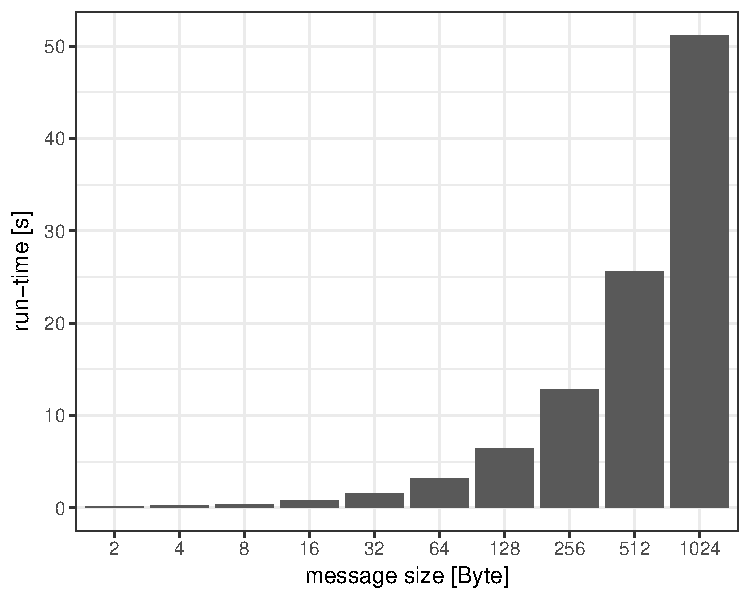
\includegraphics[width=.5\linewidth]{figures/runtime}
\caption{Run-time of algorithm X on machine Y.}
\label{fig:runtime}
\end{figure}


Table~\ref{tab:related_algorithms} shows a summary of related algorithms.

\begin{table}[ht]
\centering
\captionabove{Related algorithms and their complexity.}
\label{tab:related_algorithms}
\begin{tabular}{ll}
\toprule 
algorithm & complexity \\
\midrule
algorithm Y & $O(n)$ \\
algorithm Z & $O(n \log{n} )$ \\
\bottomrule
\end{tabular}
\end{table}

We can cite a nice book of Pinedo~\cite{Pinedo:2008vs} if we want to.
